\section{System Architecture}

\begin{figure}[h]
  \centering
  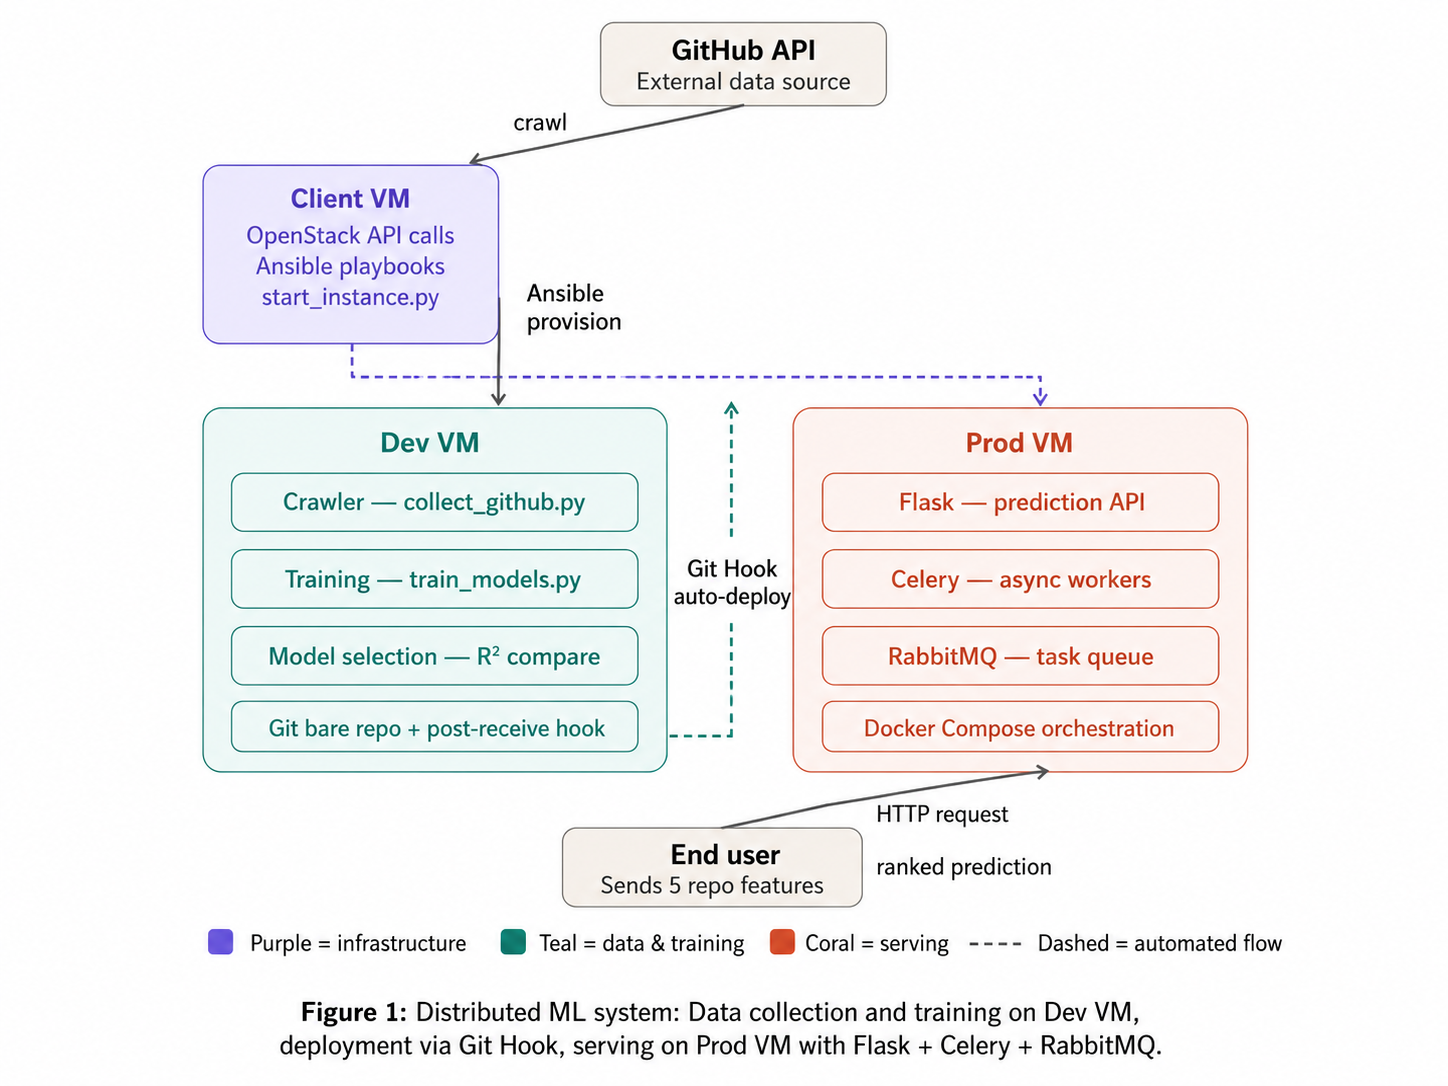
\includegraphics[width=0.95\linewidth]{figures/diagram3_combined_system_architecture_new.png}
  \caption{Distributed ML system: Data collection and training on Dev VM, deployment via Git Hook, serving on Prod VM with Flask + Celery + RabbitMQ.}
  \label{fig:combined}
\end{figure}

The architecture spans Dev (training) and Prod (serving) OpenStack VMs, enabling separation of concerns and independent scaling.

\subsection{Infrastructure and Data Collection}

Phase 1--2 provisions VMs (Ubuntu 22.04, ssc.medium flavor: 2 vCPU, 4GB RAM, 20GB storage) via OpenStack API. Phase 3 collects 2{,}000 GitHub repositories ($\geq 50$ stars) via authenticated GitHub API with rate-limit handling. Raw data includes 15 features: stargazer count, fork count, subscriber count, open issues, repository size, network count, language, wiki/pages/issues flags, topics count, age in days, and timestamps. Feature engineering selects 11 numeric/categorical attributes: 6 activity indicators (forks, subscribers, issues, size, network, age), 3 binary flags (wiki, pages, issues), 2 diversity indicators (topics, language encoding). Features are standardized via StandardScaler ($\mu=0$, $\sigma=1$) and target log-transformed: $\log(1+\text{stars})$ to normalize the right-skewed star distribution. 

Three models train on 80/20 split: (1) Linear Regression baseline, (2) SVR with RBF kernel ($C=15$, $\varepsilon=0.1$), (3) Neural Network with 3 layers (64-32-1 units, ReLU activation, 0.2 dropout). The log-transformation proves critical: star counts range from 497 to 502{,}119, causing gradient instability in raw scale; log-transform compresses this to $\log(498) \approx 6.21$ to $\log(502120) \approx 13.13$, enabling stable training.

\subsection{Deployment and Production Serving}

Phase 4 deploys via Git Hook: trained model architecture (model.json) and weights (model.weights.h5) transfer via SCP to Prod VM, triggering Docker container restart. This approach provides version-controlled model management and automated model updates. Since the Docker containers are restarted during deployment, a short service interruption may occur unless rolling deployment or multiple replicas are used. Phase 5 runs three Docker services: Flask API (port 5100, endpoints /accuracy and /predictions), RabbitMQ broker (AMQP port 5672, management UI port 15672), and Celery worker. The worker loads the trained TensorFlow model into memory for fast inference:
\begin{itemize}
  \item \textbf{get\_predictions()}: Batch inference on all 2{,}000 repositories, returns predicted vs actual stars with repository names
  \item \textbf{get\_accuracy()}: Model evaluation returning MAE metric on full dataset
\end{itemize}

Phase 6 enables horizontal scaling: \texttt{docker compose --scale worker\_1=N} creates $N$ worker replicas. Each worker independently pulls tasks from the shared RabbitMQ queue, enabling linear throughput scaling while maintaining constant per-request latency.
